\documentclass{article}

\usepackage{epsfig,graphics,psfrag,color,rotating}
\usepackage{amsmath,amsfonts,amssymb,bbm,scalefnt}


\textwidth=30cm

\def\X{\mathcal{X}}
\def\un{\mathbbm{1}}
\def\u{\mathrm{u}}

\sloppy


\begin{document}
\thispagestyle{empty}

\begin{figure}
%
\centerline{ 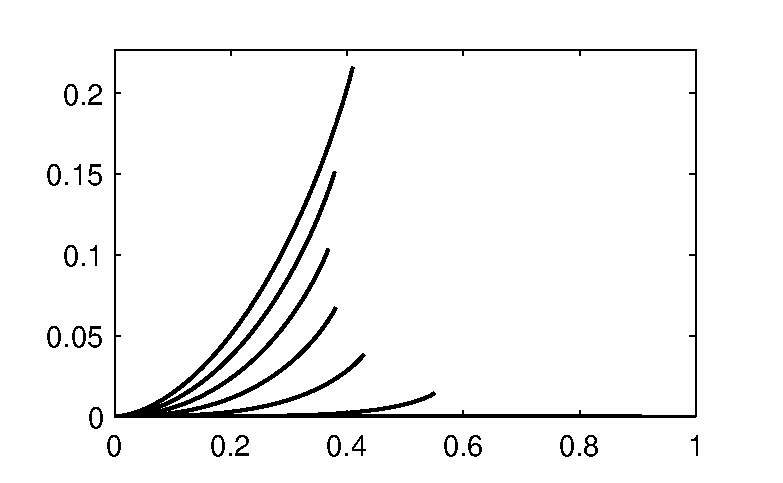
\includegraphics[width=6.5cm]{../EPS/Gamma_phi0_p1} \hspace{-5mm}
  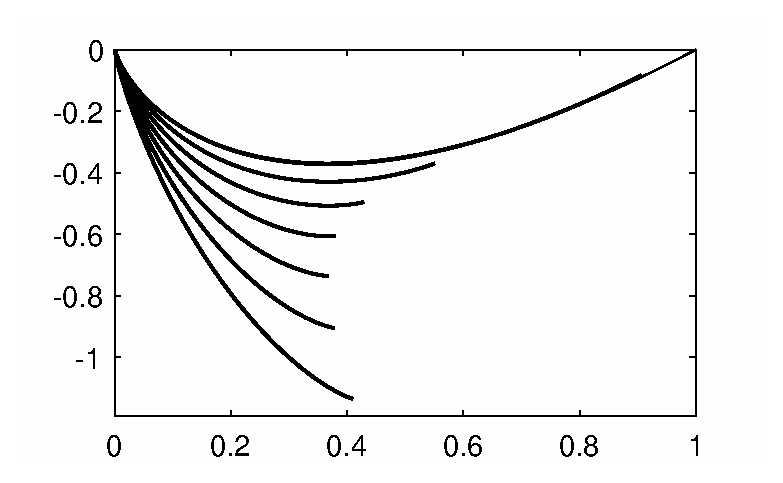
\includegraphics[width=6.5cm]{../EPS/Gamma_phi1_p1}}
%
\begin{picture}(0,0)
\put(384.5,27){\scalefont{.65}{$q = 1.02$}}
\put(353,29.5){\scalefont{.65}{$q = 1.25$}}
\put(335,39){\scalefont{.65}{$q = 1.5$}}
\put(328,50){\scalefont{.65}{$q = 1.75$}}
\put(326,64.5){\scalefont{.65}{$q = 2$}}
\put(327.5,83){\scalefont{.65}{$q = 2.25$}}
\put(332,109){\scalefont{.65}{$q = 2.5$}}
\put(340,6.5){\footnotesize $u$}
\put(243.5,39){\footnotesize \rotatebox{90}{$\phi_{0,\u}(u) - \gamma_0 - \beta u$}}
%\put(266.5,105){
%  \rotatebox{90}
%  {\scalefont{.65} $T_{k,1}(x) = x \un_{\X_k}(x)$}}
%
\put(557,110.6){\vector(1,0){25}}
\put(531,109){\scalefont{.66}{$u \, \log u$}}
\put(563,98){\scalefont{.65}{$q = 1.02$}}
\put(530,85){\scalefont{.65}{$q = 1.25$}}
\put(512,75.5){\scalefont{.65}{$q = 1.5$}}
\put(505,67.5){\scalefont{.65}{$q = 1.75$}}
\put(503.5,57.5){\scalefont{.65}{$q = 2$}}
\put(505,45){\scalefont{.65}{$q = 2.25$}}
\put(509,27.5){\scalefont{.65}{$q = 2.5$}}
\put(520,6.5){\footnotesize $u$}
\put(423.5,55){\footnotesize \rotatebox{90}{$\phi_{-1,\u}(u)$}}
%
\put(336,-6.25){(a)}
\put(516,-6.25){(b)}
\end{picture}
\end{figure}

\end{document}
